\documentclass[10pt,xcolor=svgnames]{beamer} %Beamer
\usepackage{palatino} %font type
\usepackage{tikz}
\usetikzlibrary{calc}
%\usepackage[style=verbose,backend=biber]{biblatex}
\usepackage[style=authoryear]{biblatex}
\renewcommand*{\nameyeardelim}{\addcomma\addspace}

\usefonttheme{metropolis} %Type of slides
\usefonttheme[onlymath]{serif} %font type Mathematical expressions
\usetheme[progressbar=frametitle]{metropolis} %This adds a bar at the beginning of each section.

\usepackage{appendixnumberbeamer} %enumerate each slide without counting the appendix
\setbeamercolor{progress bar}{fg=Orange!70!Coral} %These are the colours of the progress bar. Notice that the names used are the svgnames
\setbeamercolor{title separator}{fg=DarkSalmon} %This is the line colour in the title slide
\setbeamercolor{structure}{fg=black} %Colour of the text of structure, numbers, items, blah. Not the big text.
\setbeamercolor{normal text}{fg=black!87} %Colour of normal text
\setbeamercolor{alerted text}{fg=DarkRed!60!Gainsboro} %Color of the alert box
\setbeamercolor{example text}{fg=Maroon!70!Coral} %Colour of the Example block text

\def\checkmark{\tikz\fill[scale=0.4](0,.35) -- (.25,0) -- (1,.7) -- (.25,.15) -- cycle;}

\definecolor{backgroundExp}{RGB}{127.5,127.5, 127.5} %These are the colours of the background. Being this the main combination and so one. 
\setbeamercolor{palette primary}{bg = backgroundExp, fg=white}
\setbeamercolor{palette secondary}{bg=NavyBlue!50!DarkOliveGreen, fg=white}
\setbeamercolor{palette tertiary}{bg=NavyBlue!40!Black, fg= white}
\setbeamercolor{section in toc}{fg=NavyBlue!40!Black} %Color of the text in the table of contents (toc)

%These next packages are the useful for Physics in general, you can add the extras here. 
\usepackage{amsmath,amssymb}
\usepackage{slashed}
\usepackage{cite}
\usepackage{relsize}
\usepackage{caption}
\usepackage{subcaption}
\usepackage{multicol}
\usepackage{booktabs}
\usepackage[scale=2]{ccicons}
\usepackage{pgfplots}
\usepgfplotslibrary{dateplot}
\usepackage{geometry}
\usepackage{xspace}


\definecolor{mpigreen}{HTML}{007977}
\setbeamercolor{frametitle}{bg=mpigreen}

\definecolor{experimentBackground}{RGB}{127.5,127.5,127.5}

\newcommand{\themename}{\textbf{\textsc{bluetemp}\xspace}}%metropolis}}\xspace}
\titlegraphic{%
  \begin{picture}(0,0)
    \put(315,-200){\makebox(0,0)[rt]{
\includegraphics[width=1cm]{logos/logoCPI.jpeg}}}
  \end{picture}
  \begin{picture}(0,0)
    \put(280,-200){\makebox(0,0)[rt]{
\includegraphics[width=4cm]{logos/logoMPI.png}}}
  \end{picture}
  \begin{picture}(0,0)
    \put(80,-200){\makebox(0,0)[rt]{
\includegraphics[width=3cm]{logos/logoUNI.png}}}
  \end{picture}
  }
  

\title{Characterizing Temporal Dynamics of Visual Perceptual Grouping}
\author[Name]{Mehmet Yörüten \\
            \textbf{Supervised by: } Shuchen Wu, Felix Wichmann, Eric Schulz \\ } %With inst, you can change the institution they belong
\institute[uni]{\textit{M.Sc Student of Neural Information Processing} \\ University of Tübingen}
\date{} 

%References file
\addbibresource{presentationRefs.bib}
\begin{document}

\maketitle
\metroset{titleformat frame=smallcaps} %This changes the titles for small caps

\begin{frame}{Outline}
  \setbeamertemplate{section in toc}[sections numbered] %This is numbering the sections
  \tableofcontents[hideallsubsections] %You can comment this line if you want to show the subsections in the table of contents
\end{frame}


%%%%%%%%%%%%%%%%%%%%%%%%%%%%%%%%%%%%%%%%%%%%
\section{Visual Grouping}


\begin{frame}{Perceptual Grouping Retains a Hierarchical Structure}
    \begin{figure}
        \centering
        \begin{subfigure}{0.3\textwidth}
            \centering
            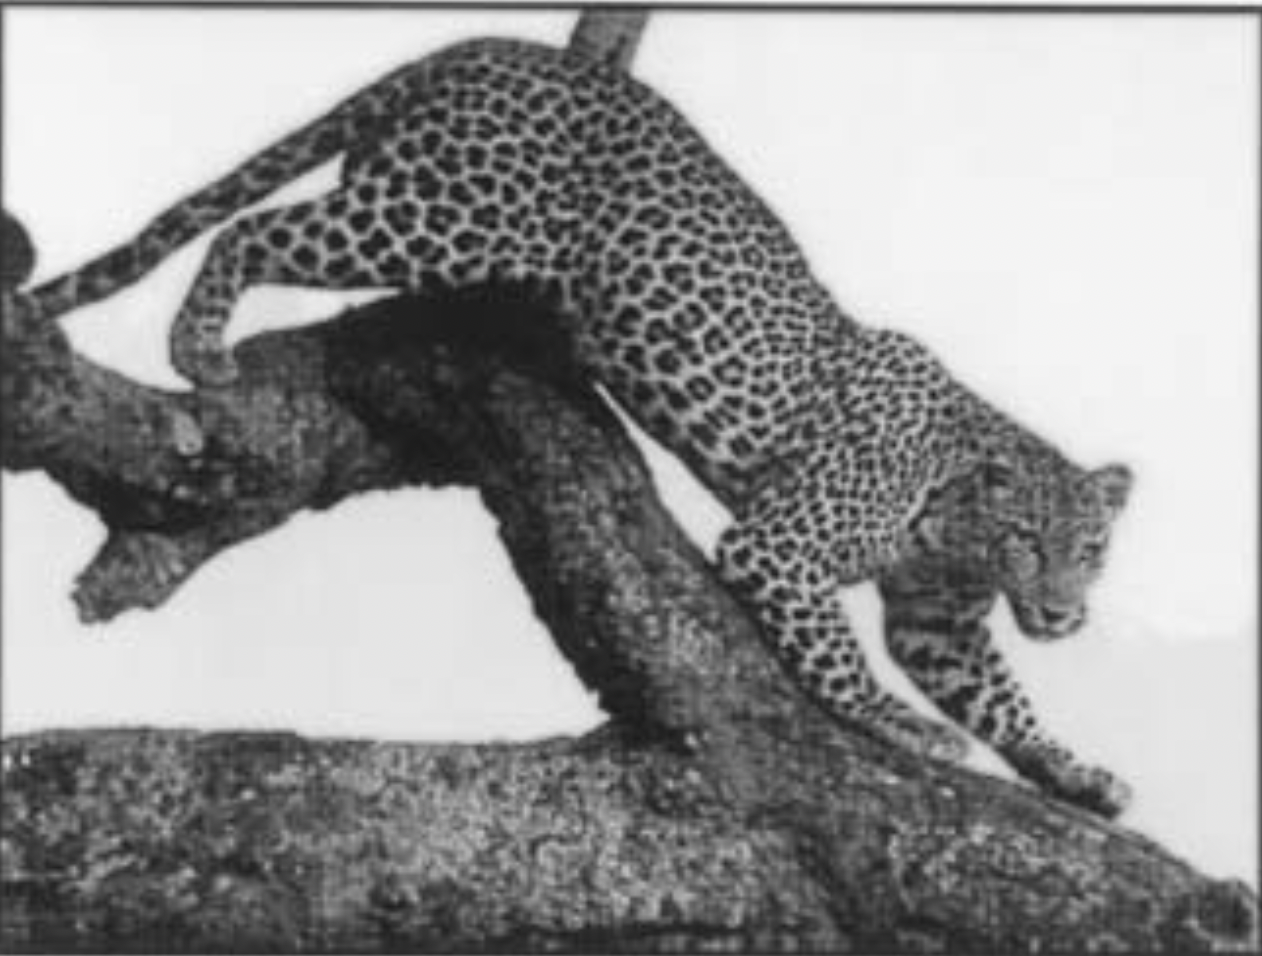
\includegraphics[width=\textwidth]{pictures/perceptualOrganization_1.png}
            \label{fig:perceptualOrg_a}
            \caption{}
        \end{subfigure}
        \hfill
        \begin{subfigure}{0.3\textwidth}
            \centering
            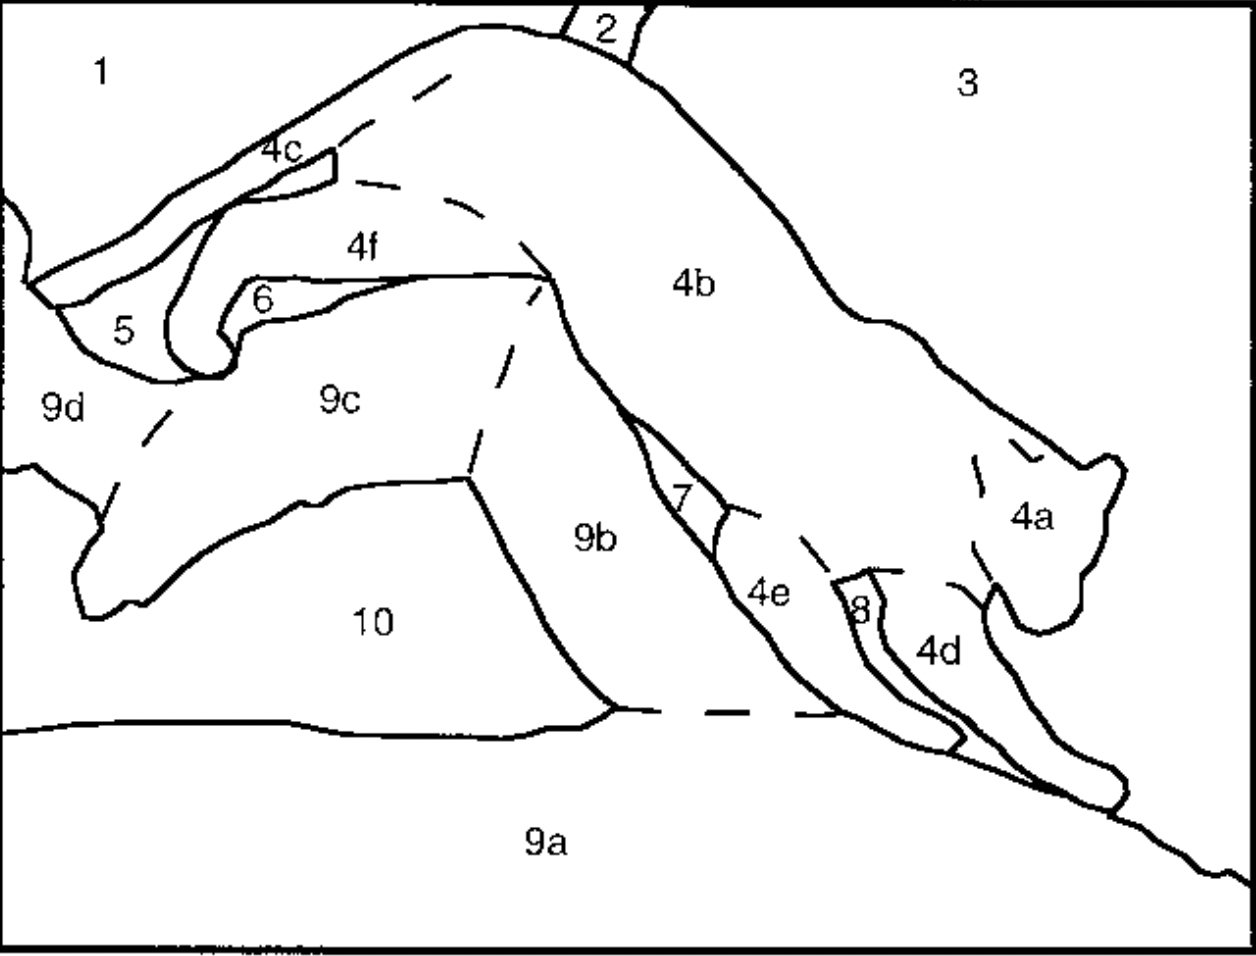
\includegraphics[width=\textwidth]{pictures/perceptualOrganization_2.png}
            \caption{}
            \label{figure:perceptualOrg_b}
        \end{subfigure}
        \hfill
        \begin{subfigure}{0.32\textwidth}
            \centering
            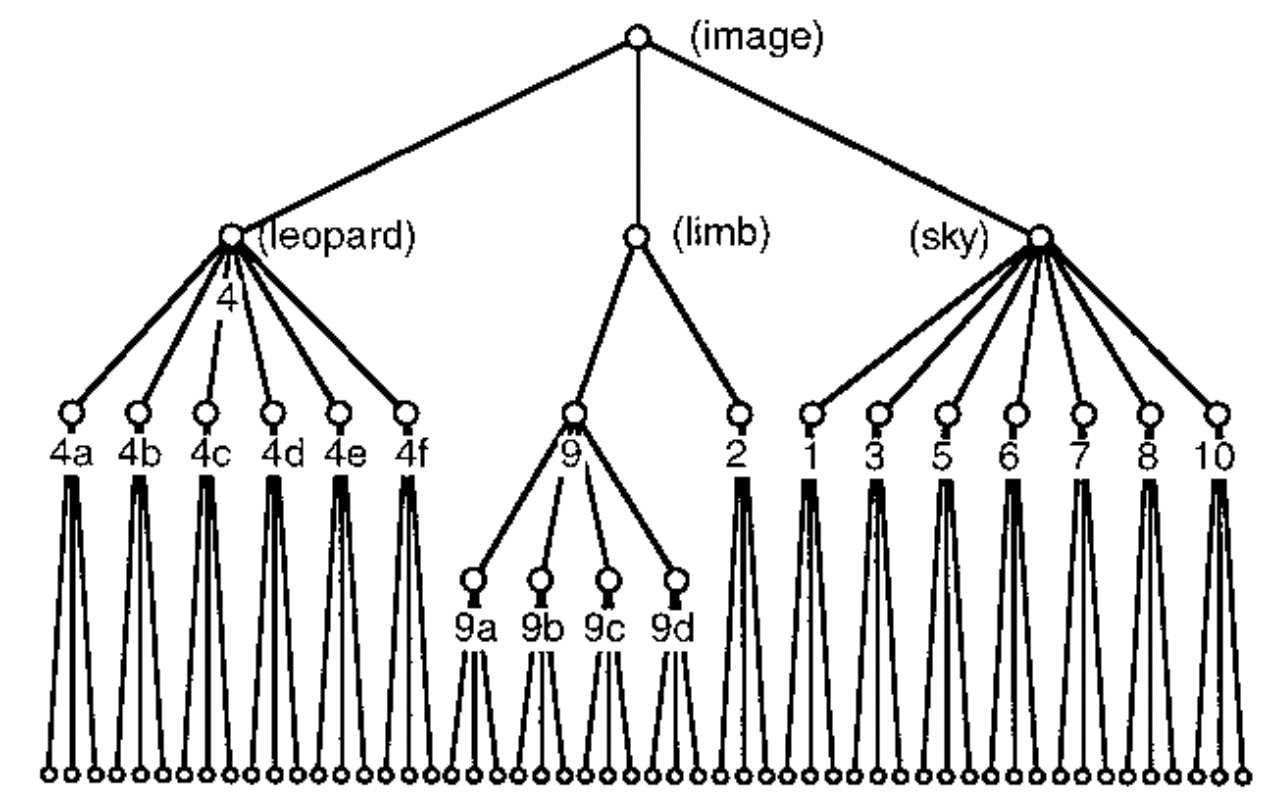
\includegraphics[width=\textwidth]{pictures/perceptualOrganization_3.png}
            \caption{}
            \label{figure:perceptualOrg_c}
        \end{subfigure}
    \caption{Perception of this image (1a) is organized into structured components (\ref{figure:perceptualOrg_b}). These structure components can be described by a hierarchical graph (\ref{figure:perceptualOrg_c}), with coarser components in the shallower layers, and finer components in deeper layers.
    
    \\
    {\footnotesize Adapted from \textcite{RN212}}
        }
    \label{fig:perceptual_org}
    \end{figure}
    
\end{frame}


\begin{frame}{Motivation}
    \begin{itemize}
        \item Grouping under inattention (Kimchi, 2009; Montoro et al.,2018)
        \item Hints for some order in perceptual grouping (Global precedence effect (Navon, 1981), Hierarchical motion structure (Gershman et al., 2015))
        \item Grouping with proximity requires time (Kurylo, 1997)
        \item Some grouping principles are superior to others (Razpurker-Apfeld & Kimchi, 2007)
    \end{itemize}

    BUT;
    \begin{itemize}
        \item Hierarchies with more than 2 groups was not well studied
        \item Effect of time on grouping with similairty in luminance is not clear
        \item A model which can approximate these relationships is missing
    \end{itemize}
\end{frame}


\begin{frame}{Motivation}

\metroset{block=fill}
\begin{exampleblock}{\textsc{Hypothesis}}
As more computational resources are allocated, perceptual grouping behavior gets refined and finer segments can be detected.
\end{exampleblock}

\begin{itemize}
    \item \textit{For cognitive scientists:} What correlates with the structure of perception, when there is no inductive bias
    \item \textit{For computer vision:} This is a spelled out property for human vision. A good computer vision system should exert similar properties.
\end{itemize}
\end{frame}

\begin{frame}{Goals}

\begin{itemize}
    \item When seeing an image without top-down influnce, is the number of cuts coming from a hierarchical graph relate to perceptual difficulty?   
    \item Does increasing exposure time alleviates the difficulty imposed by n cut?
\end{itemize}
\end{frame}


\begin{frame}{Experiment - Contrast Sensitivity}
    \begin{figure}
    \centering
        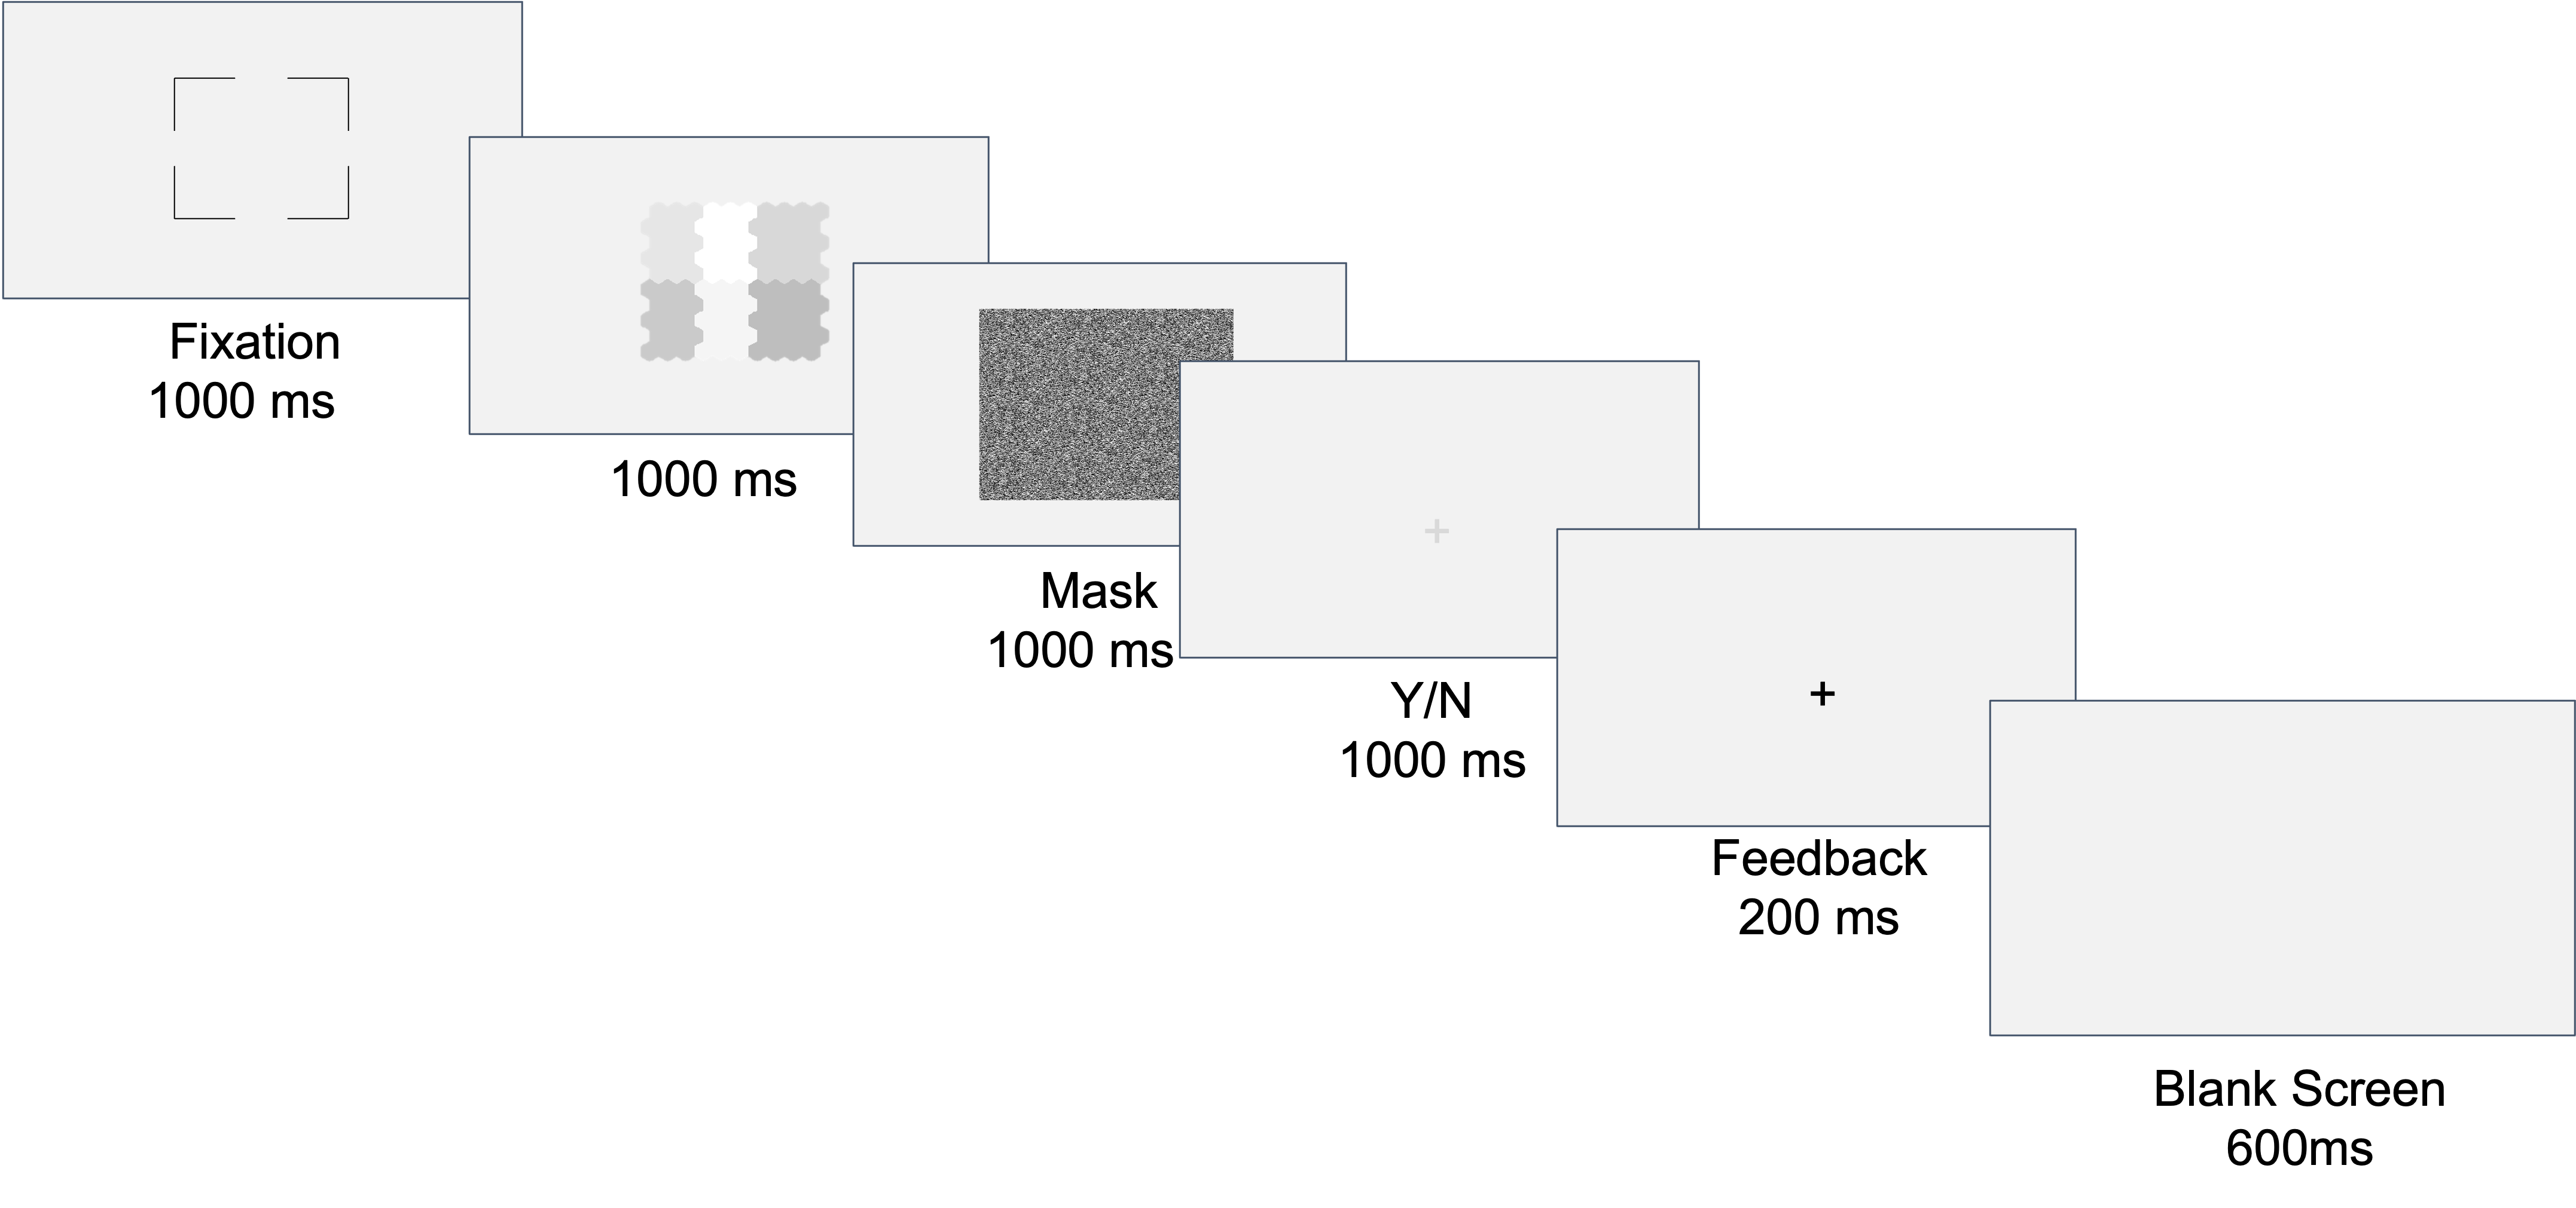
\includegraphics[width = \textwidth]{pictures/thresholdExpProcedure.png}   
    \caption{\footnotesize Estimating Individual Contrast Sensitivity}
    \end{figure}    
    \vspace{-0.5cm}
    \begin{itemize}
        \item Present 10x10 grid pattern with six different intensities
        \item Segment borders remain same
        \item Staircase Method (QUEST) to get contrast difference between segments ($\delta I$)
        \item "Did you detect 6 segments?"
    \end{itemize}
\end{frame}

\begin{frame}{Experiment}
    \begin{figure}
    \centering
        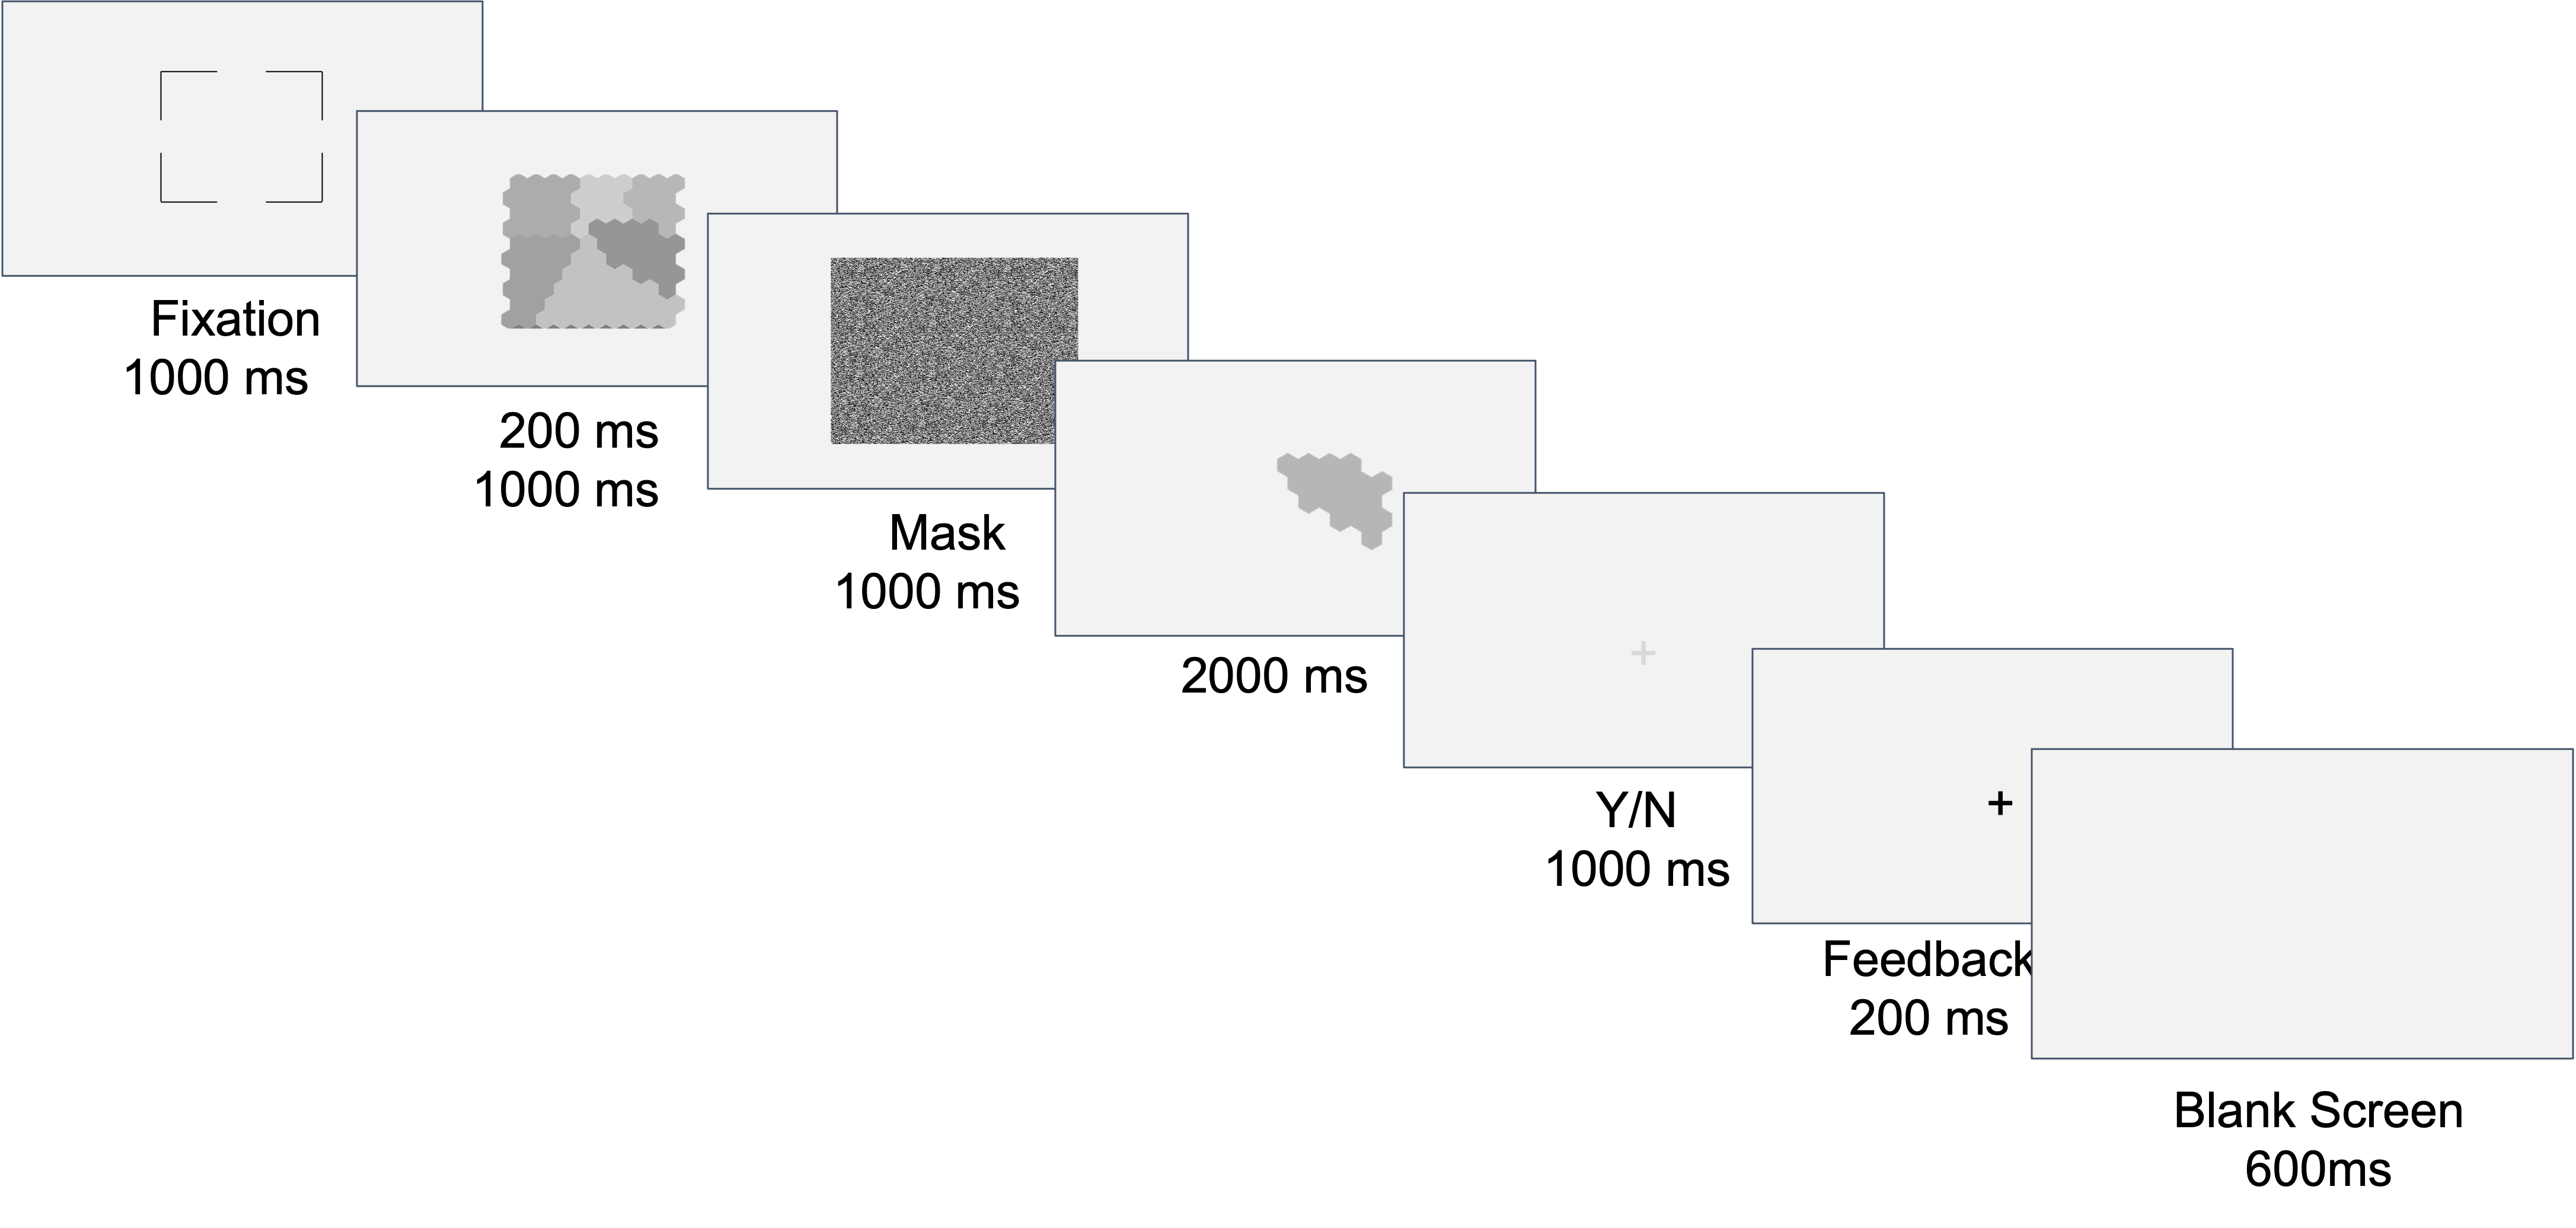
\includegraphics[width = \textwidth]{pictures/ExperimentalProcedure.png}   
    \caption{\footnotesize Experimental Procedure}
    \end{figure}    
    \vspace{-0.5cm}

    \begin{itemize}
        \footnotesize
        \item Present 10x10 grid pattern with six different intensities assigned randomly to each of groups 
        \item Present segments in average intensity value of the image
        \item Ask "Did you see the presented segment in the previously shown image?" (Y/N)
    \end{itemize}
\end{frame}
%%%%%%%%%%%%%%%%%%%%%%%%%%%%%%%%%%%%%%%%%%%%%%%%%%
\section{Initial Results}

\begin{frame}{Regressors}
    \begin{itemize}        
        \item  \textbf{Cut No:} 
        \item  \textbf{Exposure Time:}
        \item  \textbf{Segment Size:} Total number of hexagons in a segment
        \item  \textbf{Seg. Dist:} Presented segment’s distance to the center of the image
        \item  \textbf{Intensity Difference:} Average image intensity – target segment intensity in the image
        \item  \textbf{Ncut Value:} Information regarding the difficulty of the partitioning
        \item  \textbf{Highest Similarity:} 
    \end{itemize}
\end{frame}

\begin{frame}{Results - Test}
    \footnotesize  \it{glm(correct $\sim$ 1 + cutNo*expTime , family = "binomial")} \\
    \begin{figure}        
        \hspace*{-0.6cm} 
        \centering
        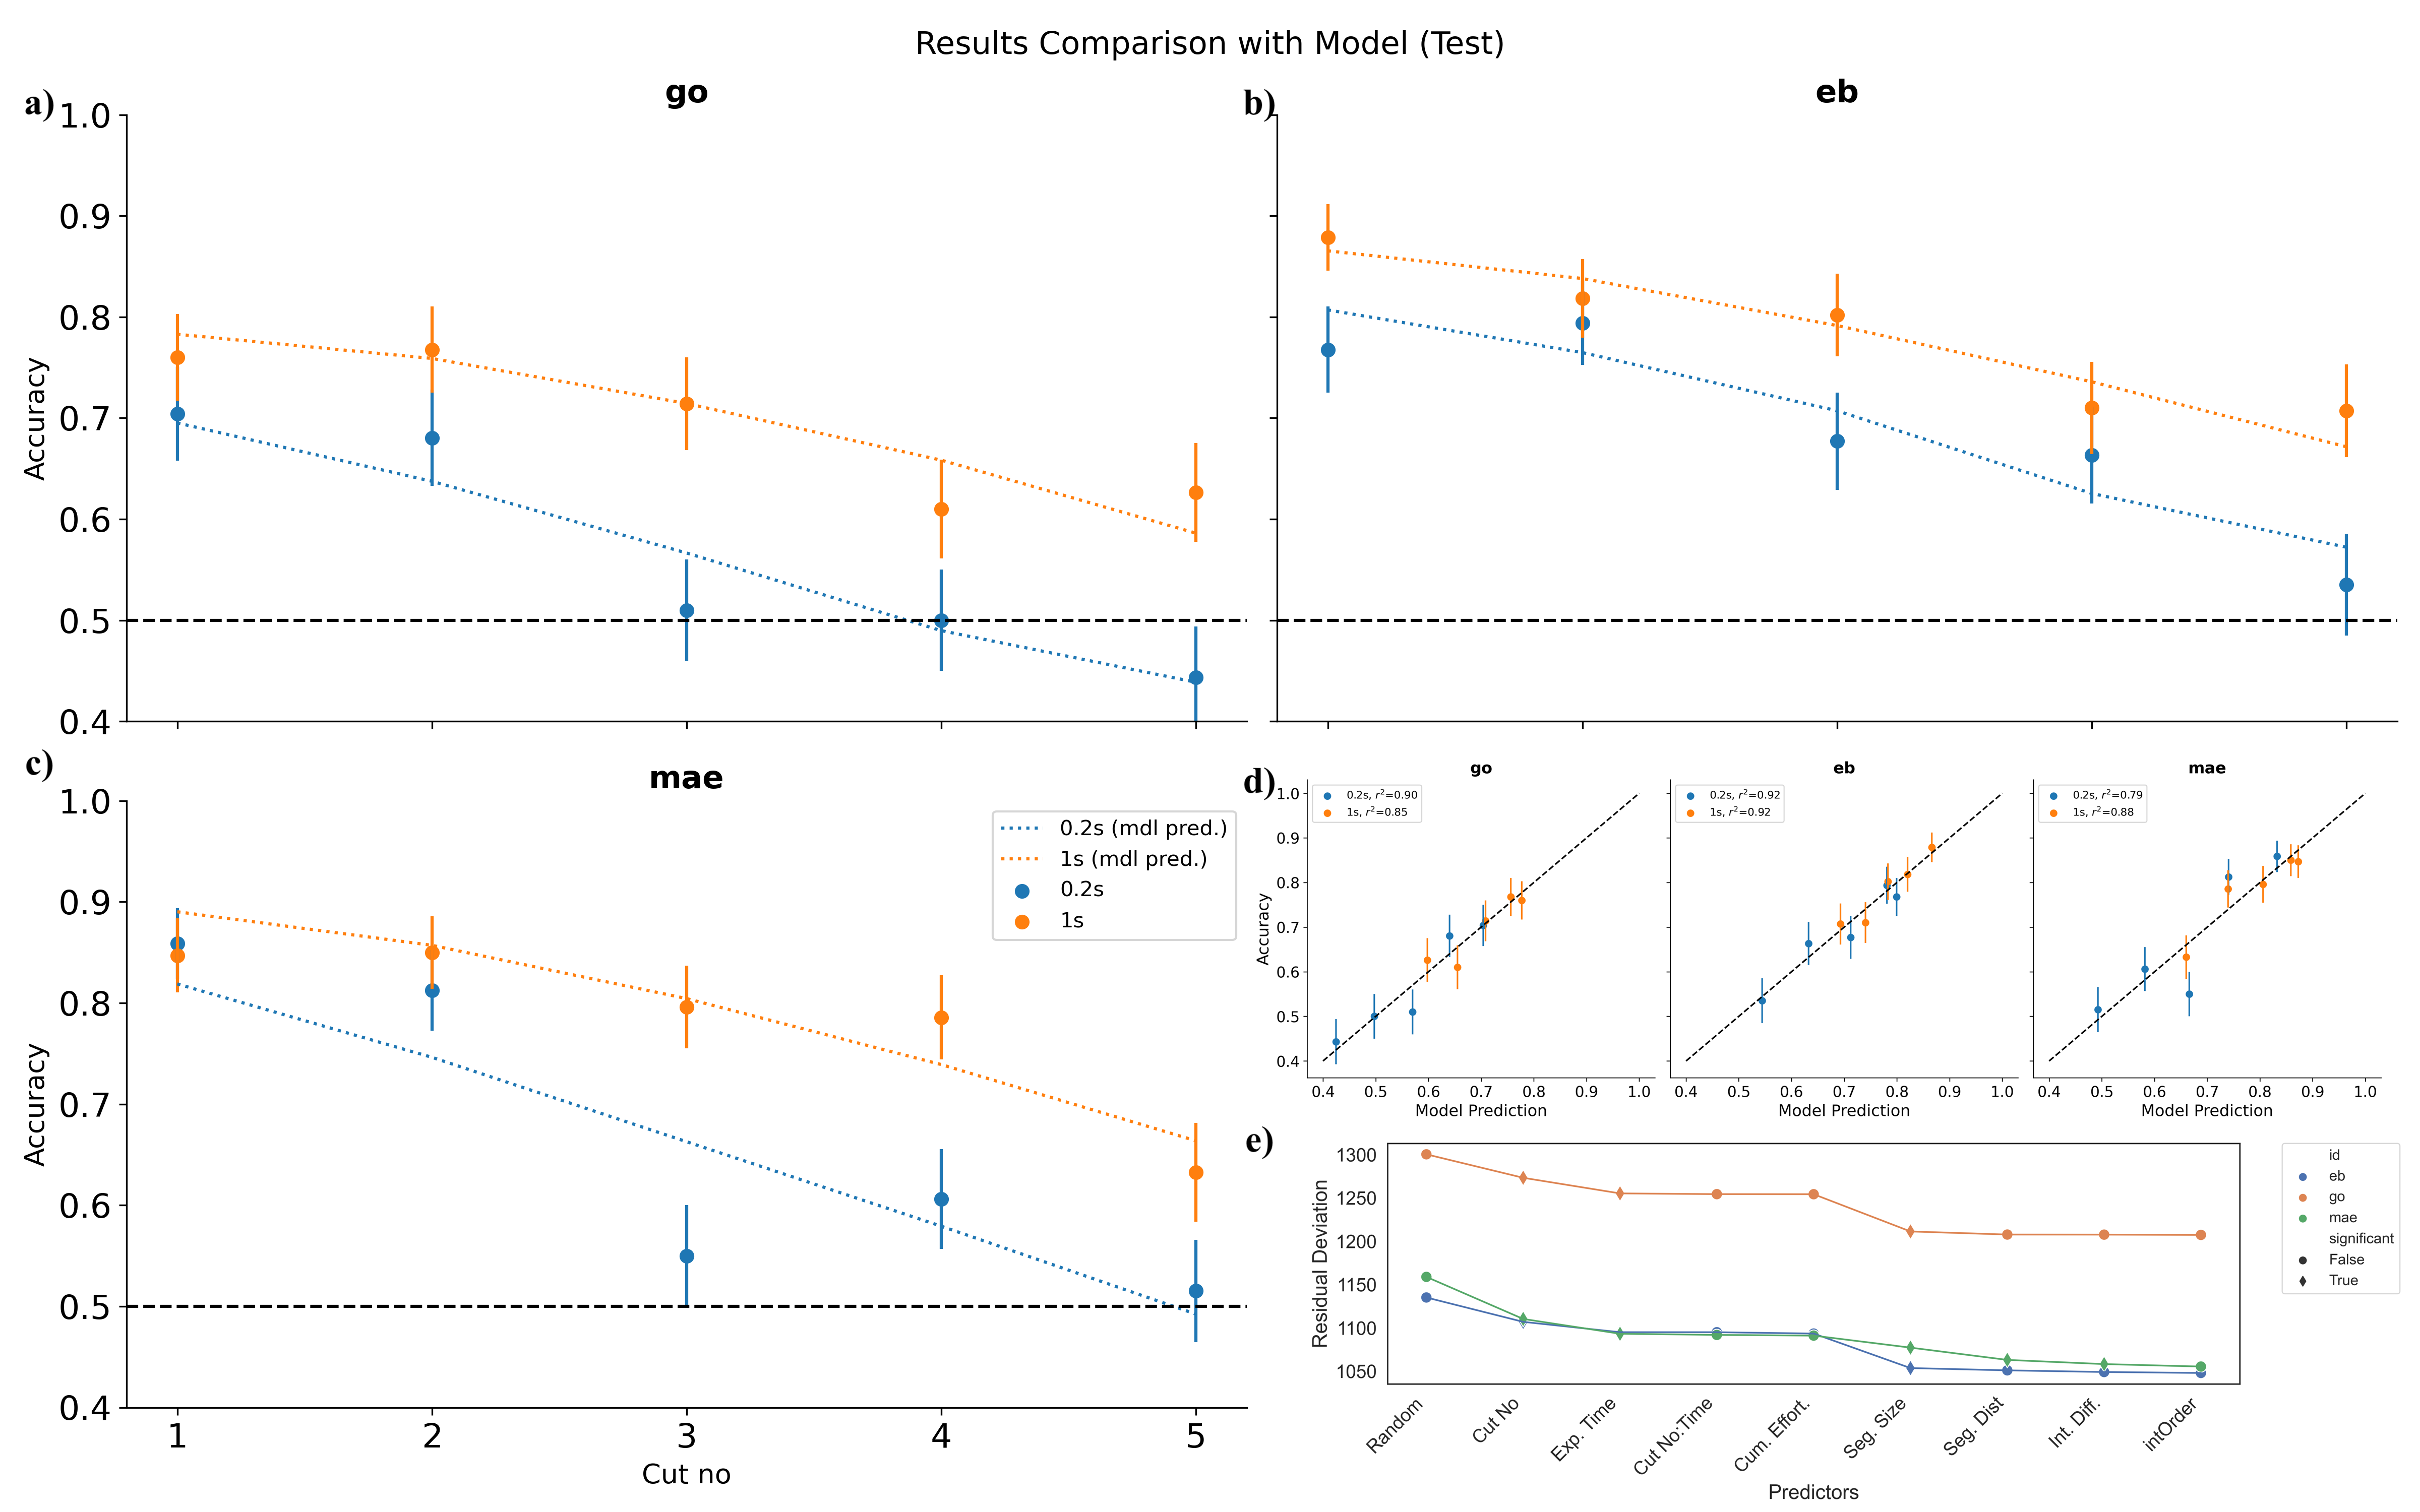
\includegraphics[width = 1.1\textwidth]{results/test_all.png}    \label{fig:test_all}
    \end{figure}
\end{frame}

\begin{frame}{Results - Control}
    \footnotesize  \it{glm(correct $\sim$ 1 + similarityScore + expTime + segCentDist + segSize, family = "binomial")} \\
    \begin{figure}        
        \hspace*{-0.6cm} 
        \centering
        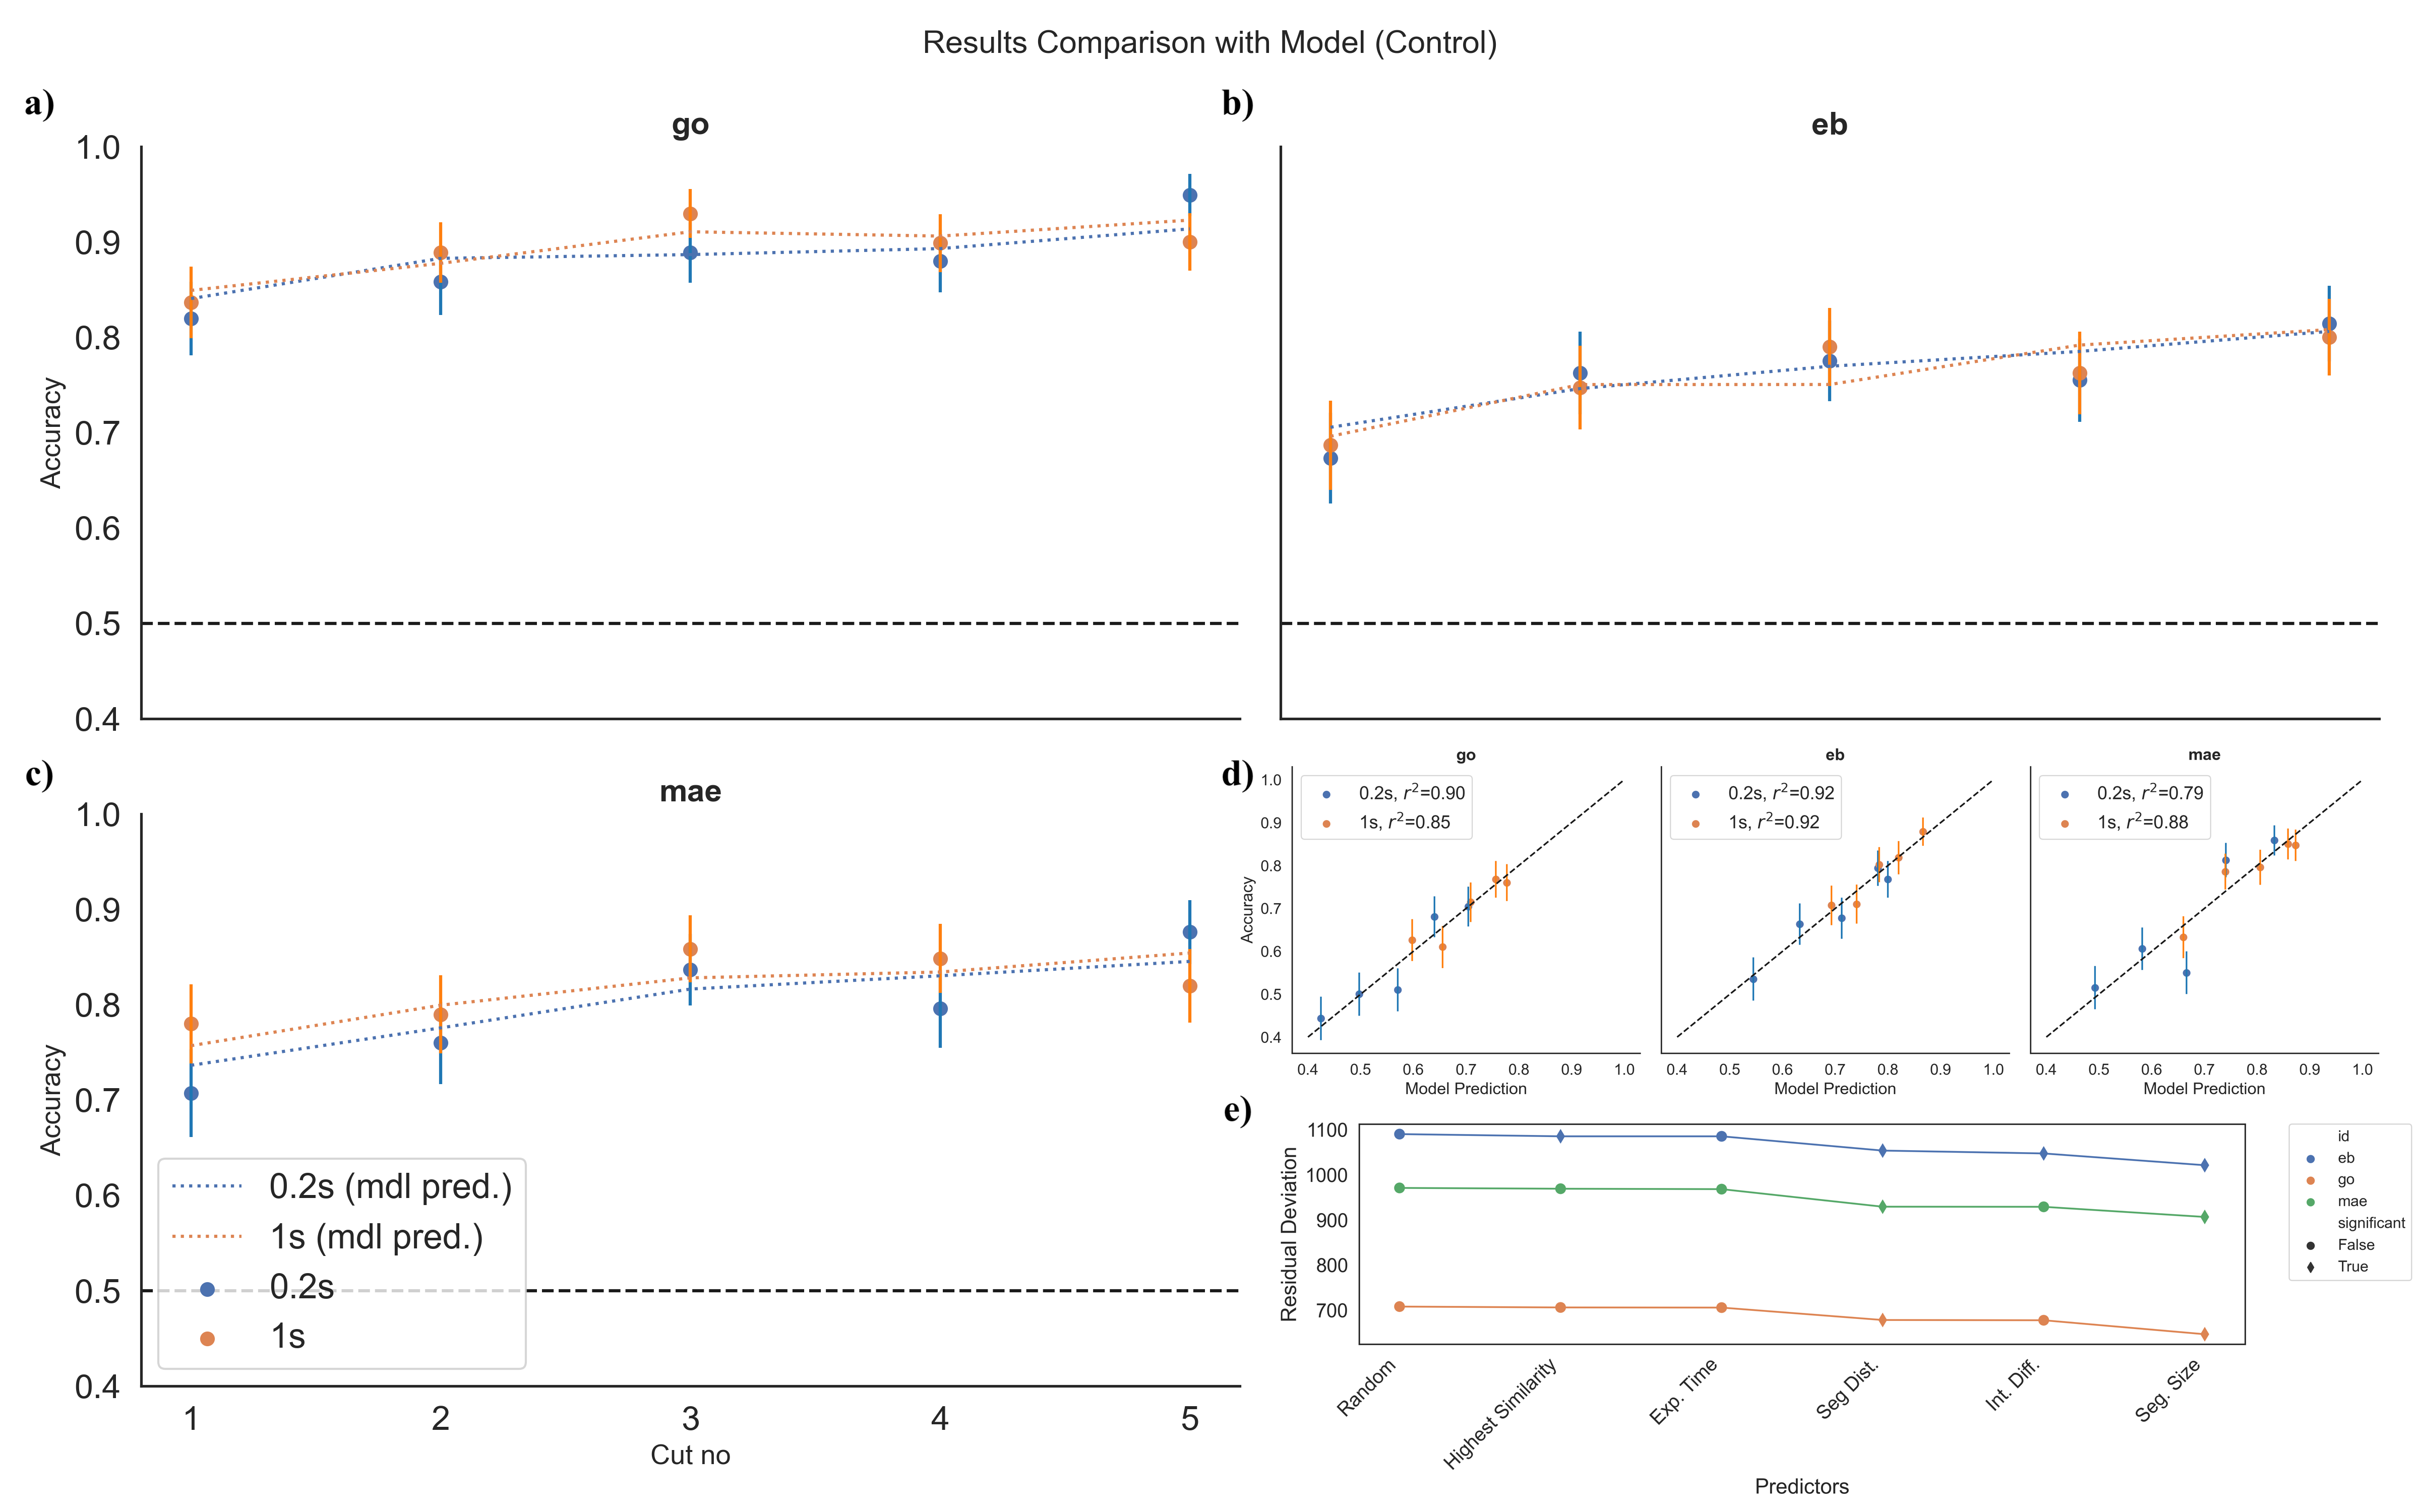
\includegraphics[width = 1.1\textwidth]{results/cntrl_all.png}    \label{fig:cntrl_all}
    \end{figure}
\end{frame}

\begin{frame}{Results - Psychometric Functions}
    \begin{figure}        
        \hspace*{-0.4cm} 
        \centering
        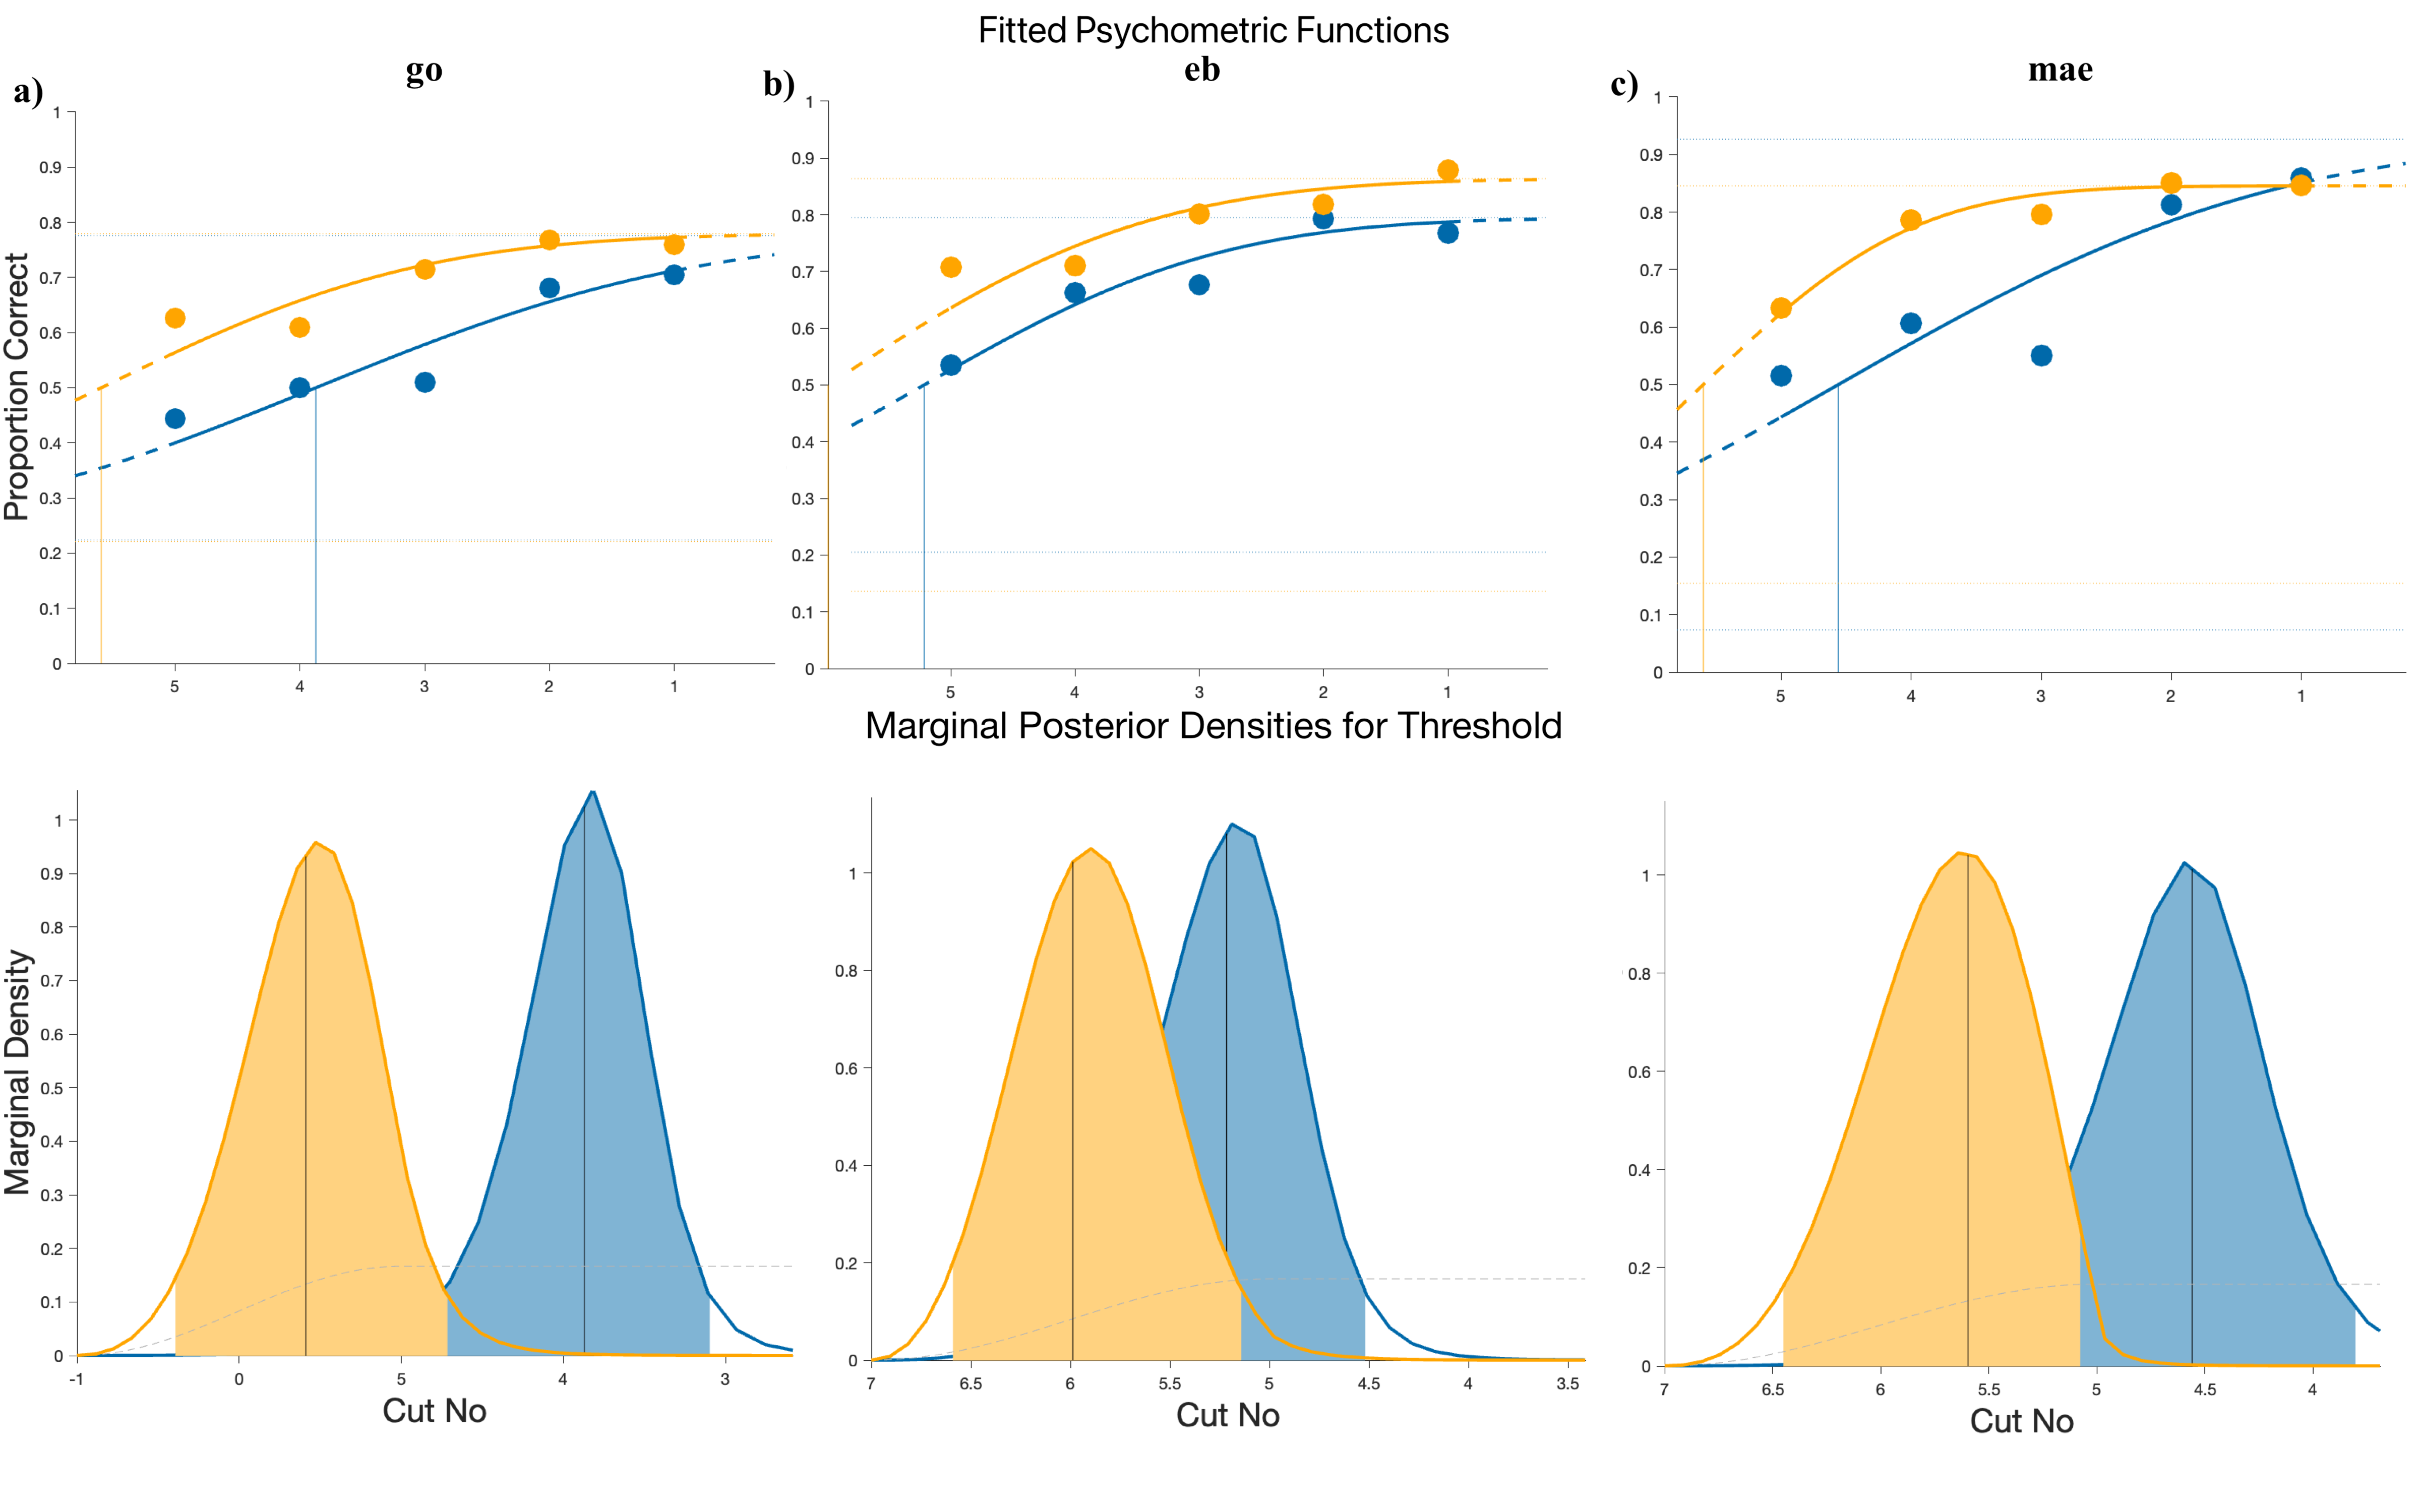
\includegraphics[width = 1.1\textwidth]{results/test_psych.png}    \label{fig:psych_fit}
    \end{figure}
\end{frame}


\begin{frame}{Results}
    \begin{figure}
        \centering
        \begin{subfigure}{0.32\textwidth}
            \centering
            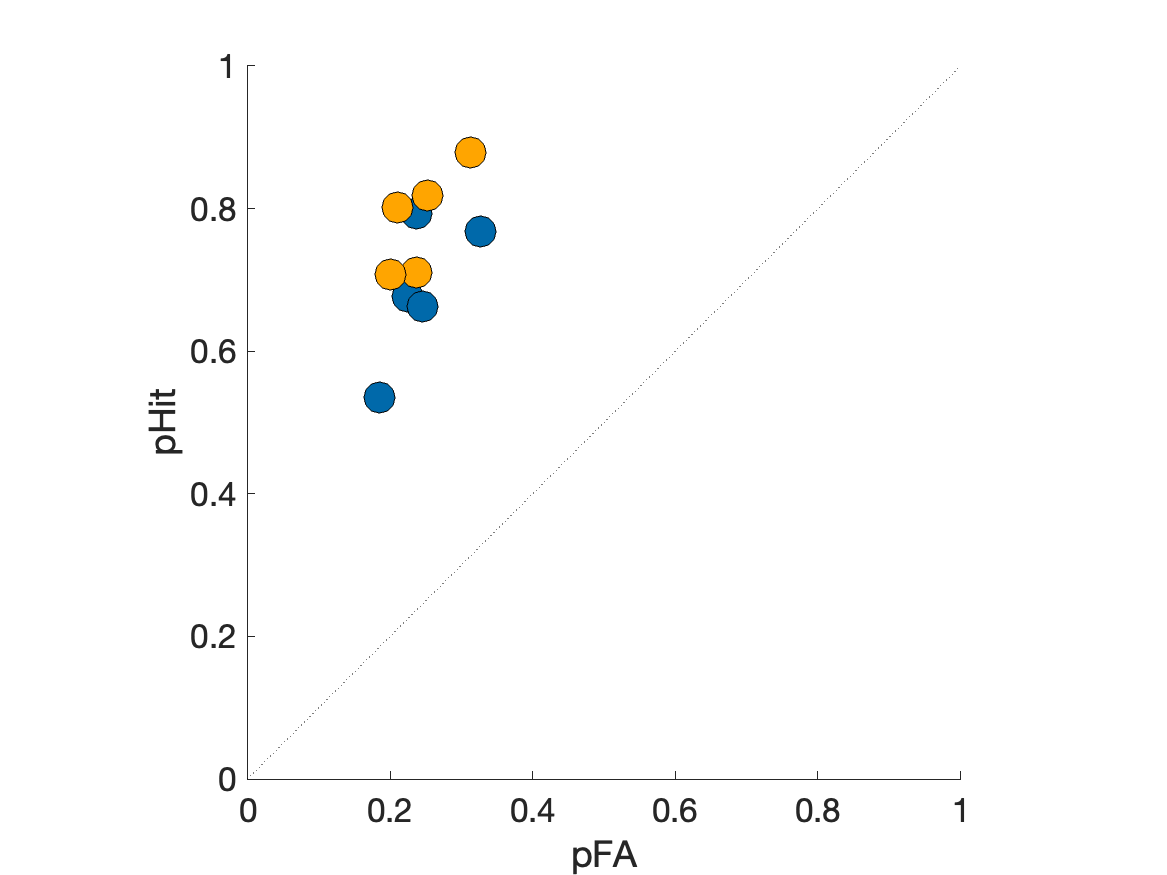
\includegraphics[width=\textwidth]{results/eb_roc.png}
            \label{figure:eb_roc}
            \caption{eb}
        \end{subfigure}
        \hfill
        \begin{subfigure}{0.32\textwidth}
            \centering
            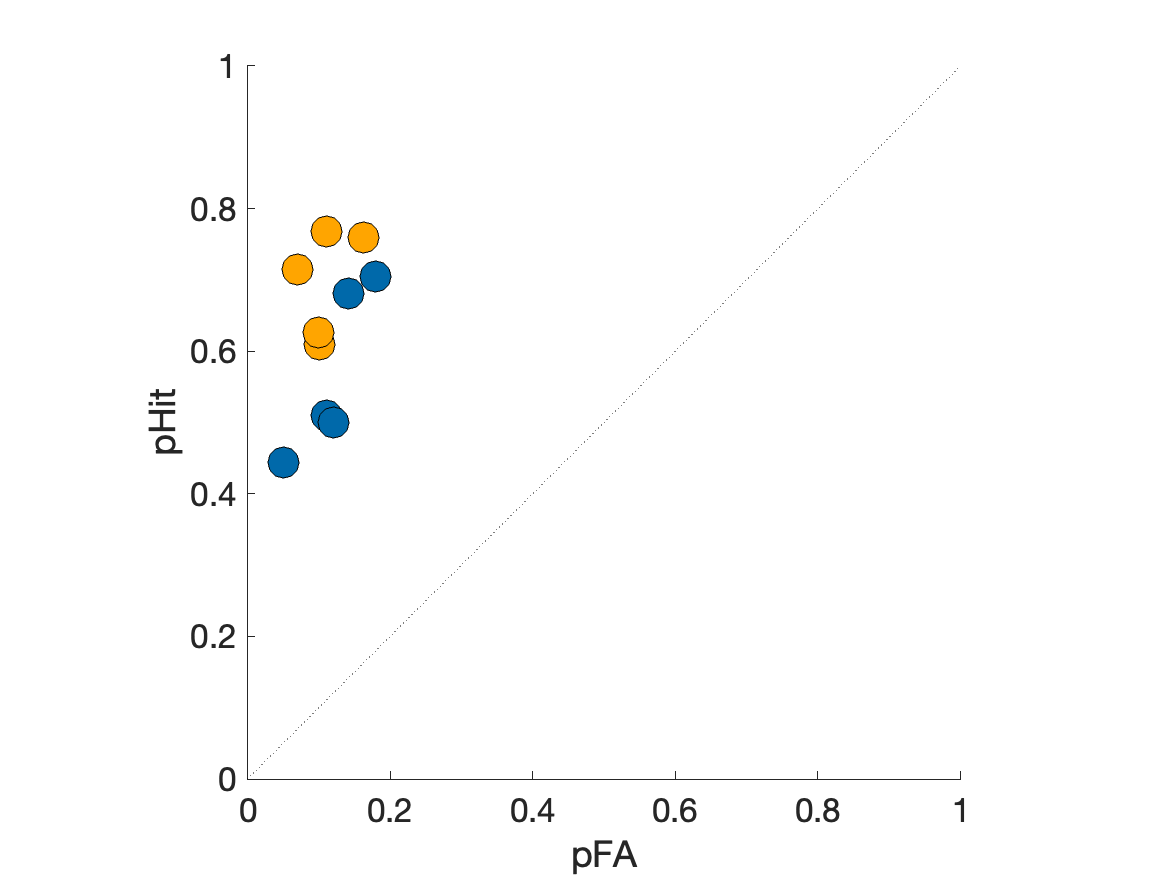
\includegraphics[width=\textwidth]{results/go_roc.png}
            \caption{go}
            \label{figure:go_roc}
        \end{subfigure}
        \hfill
        \begin{subfigure}{0.32\textwidth}
            \centering
            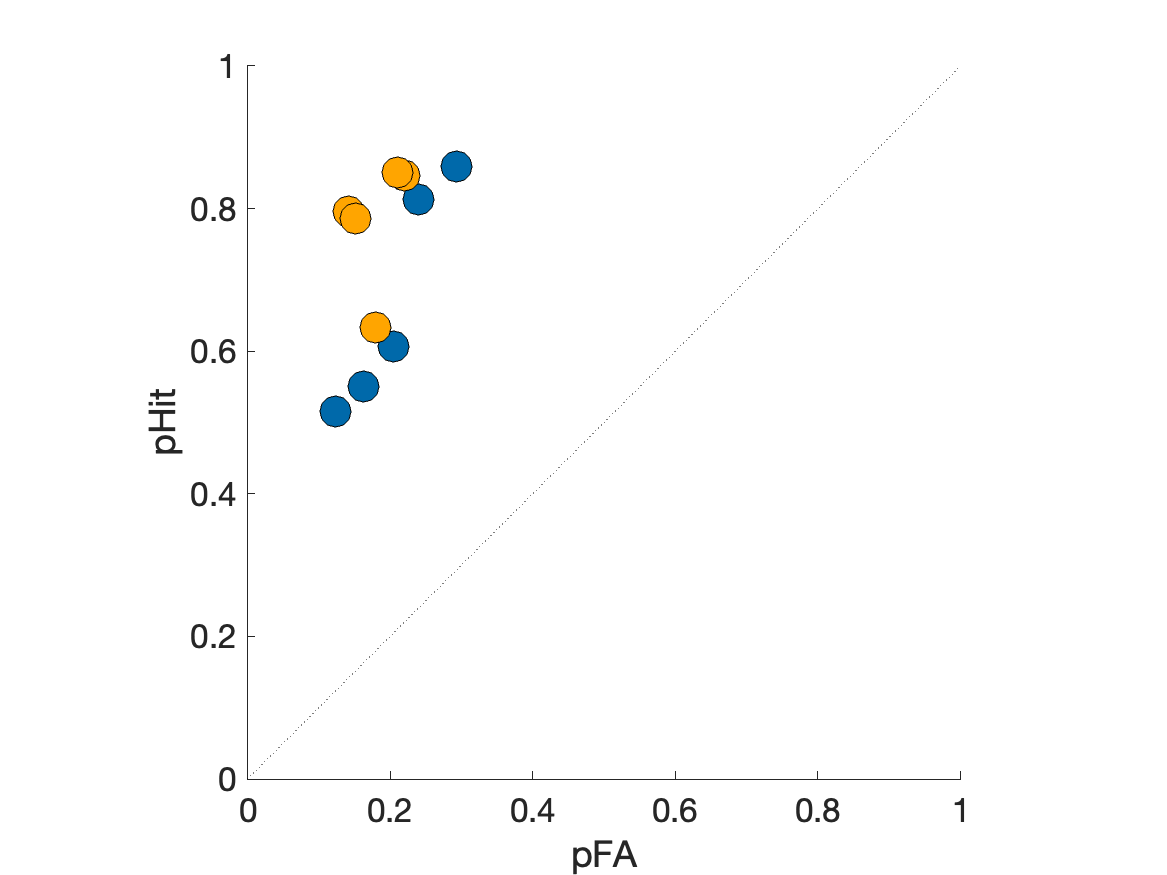
\includegraphics[width=\textwidth]{results/mae_roc.png}
            \caption{mae}
            \label{figure:mae_roc}
        \end{subfigure}   
    \label{fig:rocs}
    \end{figure}
    
\end{frame}

%%%%%%%%%%%%%%%%%%%%%%%%%%%%%%%%%%%%%%%%%%%%%%%%%%
\section{Findings and Further Directions}
\begin{frame}{Summary}
    \begin{itemize}
        \item Is the number of cuts coming from a hierarchical graph relate to perceptual difficulty?  \checkmark
            \begin{itemize}
                \item Difficulty of identifying image segments increased linearly 
            \end{itemize}        
        \item Does increasing exposure time alleviates the difficulty imposed by n cut? \checkmark
            \begin{itemize}
                \item Given more exposure time, the perceptual difficulty is alleviated.
            \end{itemize}              
        \item If the first partitionings of the image can be done with the limited resources (short exposure time), can we observe no difference between exposure times?
            \begin{itemize}
                \item Partially.            
            \end{itemize}  
    \end{itemize}
\end{frame}

\end{document}
